\section{Empirical Validation of the Lipschitz Assumption}
\label{app:lipschitz}
% ============================================================
This section provides empirical support for~\cref{asm:lip} by measuring the relationship between activation distance and change in concept generation probability under natural prompt variations, and verifying that the observed relationship is consistent with a Lipschitz bound with a small empirical constant.

\paragraph{Setup.}
For each of the ten concepts in~\cref{app:activation_regions}, we construct a set of prompt pairs $(p_b, p_v)$ where $p_b$ is a base prompt containing the concept and $p_v$ is a variant prompt obtained by one of four perturbations at increasing semantic distance:
\begin{itemize}
    \item \emph{Synonym substitution:} replacing the concept word with a close synonym (e.g., \texttt{horse} $\to$ \texttt{stallion});
    \item \emph{Scene change:} altering the background or setting while preserving the concept (e.g., ``in a field'' $\to$ ``on a beach'');
    \item \emph{Related concept:} substituting a semantically related concept (e.g., \texttt{horse} $\to$ \texttt{pony});
    \item \emph{Unrelated concept:} substituting an unrelated concept (e.g., \texttt{horse} $\to$ \texttt{castle}).
\end{itemize}
For each pair, we extract cross-attention activations at \texttt{mid\_block.attentions.0} (step $t^*{=}25$) and compute the activation distance $\|\boldsymbol{\Phi}_\theta(p_v) - \boldsymbol{\Phi}_\theta(p_b)\|_2$. We then generate images from each prompt and compute the concept generation probability $P(p)$ using a CLIP-based classifier aligned to the base concept. The quantity of interest is the pair $\bigl(\|\Phi_\theta(p_v) - \Phi_\theta(p_b)\|_2,\;|P(p_v) - P(p_b)|\bigr)$.

\Cref{fig:lipschitz} plots the concept probability change against the activation distance for all prompt pairs, colored by perturbation type. Two patterns emerge. First, the four perturbation types occupy approximately nested bands of activation distance, with synonyms producing the smallest displacements, scene changes and related-concept substitutions producing intermediate displacements, and unrelated-concept substitutions producing the largest. Second, the change in concept probability scales roughly linearly with activation distance within each band, with no prompt pair exceeding a bound of the form $|P(p_v) - P(p_b)| \leq \hat{L} \,\|\Phi_\theta(p_v) - \Phi_\theta(p_b)\|_2$ for empirical constant $\hat{L} \approx 0.174$.

% \ali{we should be careful that it doesn't seem like we are suggusting these specific values as general values, and they are specific to this example.}
We emphasize that the empirical constant $\hat{L}$ should be read as a conservative upper bound for this specific layer, timestep, and set of concepts, not as a universal property of Stable Diffusion. Varying the probe layer, the timestep, or the CLIP classifier would likely change the numerical value. The claim we extract from this measurement is weaker and more robust: the concept probability mapping is empirically smooth as a function of activation distance, with no observed violations of the Lipschitz condition across hundreds of prompt pairs spanning four perturbation types. This is the regularity our proof requires. For illustration, combining $\hat{L} \approx 0.174$ with $\varepsilon = 0.05$ yields a minimum displacement bound of $\Delta \geq (1-\varepsilon)/\hat{L} \approx 5.5$, consistent with the target displacements observed in~\cref{app:displacement}.

\begin{figure}[t]
\centering
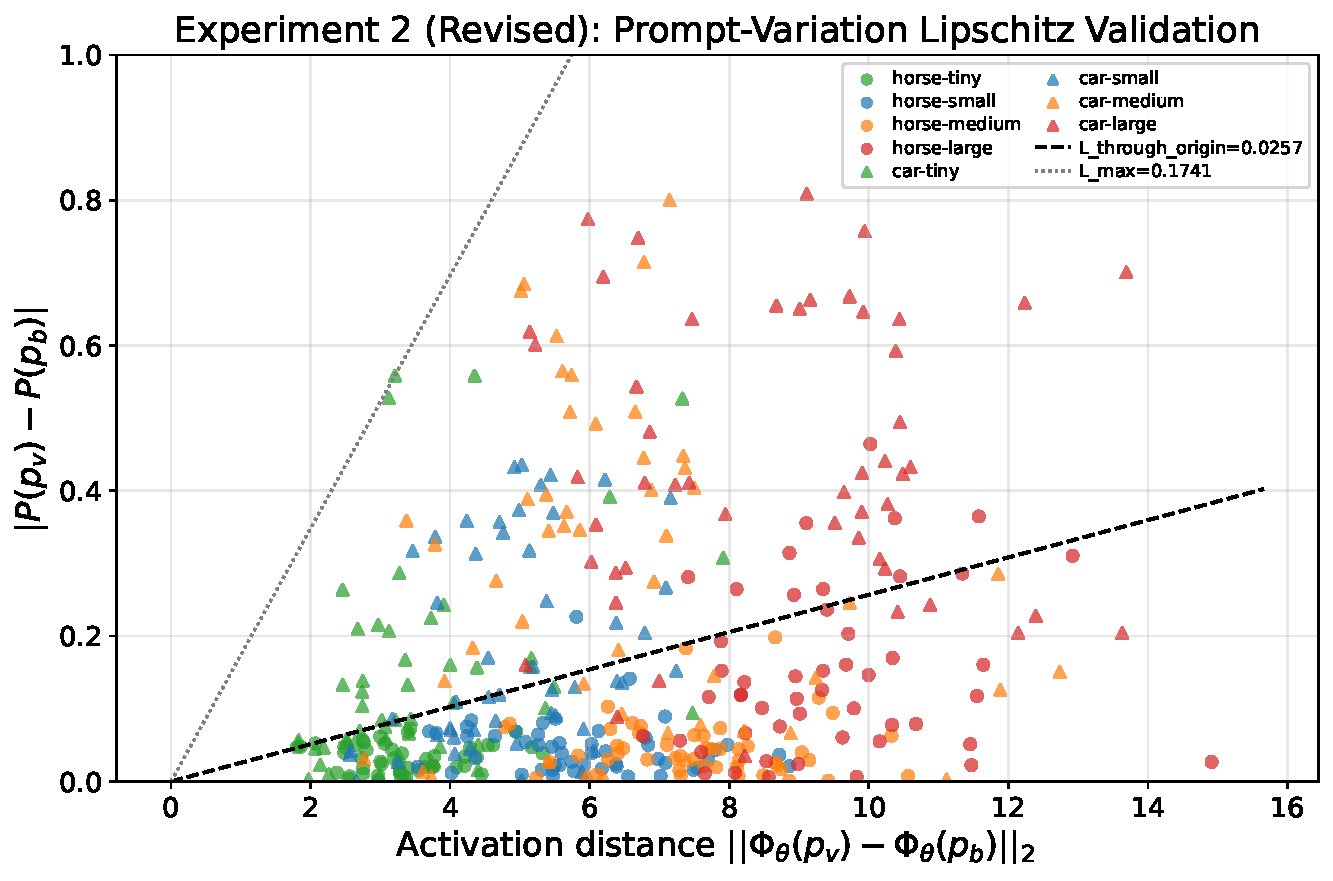
\includegraphics[width=0.85\linewidth]{img/fig_lipschitz.pdf}
\caption{
Lipschitz validation via prompt variation. Each point is a (base, variant) prompt pair; the $x$-axis shows activation distance and the $y$-axis shows the change in CLIP-based concept probability. Points are colored by semantic distance from the base prompt (green: synonyms; blue: scene changes; orange: related concepts; red: unrelated concepts). All points lie below the empirical bound $\hat{L} = 0.174$ (dotted line), supporting~\cref{asm:lip}.
}
\label{fig:lipschitz}
\end{figure}